\documentclass[handout]{beamer}
\usepackage{multicol}
\everymath{\displaystyle}
\mode<presentation>
{\usetheme{Warsaw}\setbeamercovered{dynamic}}
\usecolortheme{crane}
\usepackage{beamerfoils}
\pgfdeclareimage[height=1in]{university-logo}{ISULogo}
\logo{\pgfuseimage{university-logo}}
\setbeamertemplate{navigation symbols}{}
\title[\S4]{Section 4\\Expectation}
\author{Dr Marcus Bishop}
\subject{Math 104}
\beamerdefaultoverlayspecification{<+->}
\theoremstyle{definition}
\newtheorem{remark}{Remark}
\newtheorem{impact}{Impact}
\newtheorem{notation}{Notation}
\usepackage{arev}
\begin{document}
\begin{frame}\titlepage\end{frame}
\LogoOff

\begin{frame}{Numerical outcomes}
Section deals with experiments
that have \alert{numerical outcomes}
\begin{example}
Following experiments have numerical outcomes
\begin{itemize}
\item Number of minutes randomly selected
customer waits in line at Hy-Vee
\item Number of olives in jar
\item Number of minutes randomly selected
student takes to complete quiz
\item Lifetime in hours of light bulb
\end{itemize}
\end{example}
\end{frame}

\begin{frame}
\begin{example}
Following experiments \alert{don't} have numerical outcomes
\begin{itemize}
\item Flipping coin
\item Color of shirt randomly selected student wearing
\item Day of week my package from Amazon arrives
\end{itemize}
\end{example}
\begin{remark}
\begin{itemize}
\item Outcomes of rolling die might or might not be numerical
\item Outcomes $1,2,3,4,5,6$  often have no significance as numbers
\item Can often be replaced with non-numerical outcomes,
such as colors, letters, etc.
\item In contrast, in Monopoly outcome of rolling dice
determines \alert{number} of spaces to advance
\end{itemize}
\end{remark}
\end{frame}

\begin{frame}{Expectation}
\begin{definition}
\begin{itemize}
\item Suppose experiment has outcomes $E_1,E_2,\ldots$
\item $P_1=P\left(E_1\right)$
\item $P_2=P\left(E_2\right),\ldots$
\item Then
\[P_1E_1+P_2E_2+\cdots\]
the \alert{expectation} of experiment
\end{itemize}
\end{definition}
\begin{remark}
\begin{itemize}
\item Expectation gives
\alert{expected value} of experiment \alert{in long run}
\item Doesn't give exact value we expect
next time experiment repeated
\item Expectation used in same way averages used
\end{itemize}
\end{remark}
\end{frame}

\begin{frame}{Time to take quiz}
\begin{itemize}
\item Time it took calculus students to complete quiz
shown in table:
\[\begin{array}{r|ccc}
\text{Time in minutes}&5&8&40\\\hline
\text{Number of students}&25&13&2
\end{array}\]
\item So average time
\[\frac{5\left(25\right)+8\left(13\right)+40\left(2\right)}{40}
\only<+->{=\frac{309}{40}}
\only<+->{\approx 7.73}\]
\item But observe that
\[\frac{5\left(25\right)+8\left(13\right)+40\left(2\right)}{40}
=5\left(\frac{25}{40}\right)+8\left(\frac{13}{40}\right)
+40\left(\frac{2}{40}\right)\]
\item So average and expectation coincide in this example
\end{itemize}
\end{frame}

\begin{frame}{Multiple choice strategy (Example 2)}
\begin{itemize}
\item Suppose multiple choice question has five answer choices
\item $2$~points for correct response
\item $-1/2$~point for incorrect response
\item $0$~points for not answering
\item Should you guess if you don't know answer?
\item Outcomes:
\begin{itemize}
\item $2$ occurs with probability $1/5$ when correct answer chosen
\item $-1/2$ occurs with probability $4/5$ when incorrect answer chosen
\end{itemize}
\item So $2\cdot\frac{1}{5}+\left(-\frac{1}{2}\right)\frac{4}{5}
\only<+->{=\frac{2}{5}-\frac{4}{10}}
\only<+->{=\frac{4}{10}-\frac{4}{10}}
\only<+->{=0}$ the expectation
\item Conclusion: guessing doesn't hurt \alert{in this case}
\end{itemize}
\end{frame}

\begin{frame}
\begin{itemize}
\item Suppose multiple choice question has five answer choices
\item \alert{$1$~point} for correct response
\item $-1/2$~point for incorrect response
\item $0$~points for not answering
\item Should you guess if you don't know answer?
\item Outcomes:
\begin{itemize}
\item $1$ occurs with probability $1/5$ when correct answer chosen
\item $-1/2$ occurs with probability $4/5$ when incorrect answer chosen
\end{itemize}
\item So $1\cdot\frac{1}{5}+\left(-\frac{1}{2}\right)\frac{4}{5}
\only<+->{=\frac{1}{5}-\frac{4}{10}}
\only<+->{=\frac{1}{5}-\frac{2}{5}}
\only<+->{=-\frac{1}{5}}$ the expectation
\item Conclusion: guessing a bad idea!
\end{itemize}
\end{frame}

\begin{frame}{Card game (Exercise 14)}
\begin{itemize}
\item Mike and Dave play following game:
\item Mike randomly selects card
\item If $\clubsuit$ selected Dave gives Mike $\$4$
\item Otherwise Mike gives Dave $\$2$
\item Mike's expected proceeds:
\[4\left(\frac{1}{4}\right)+\left(-2\right)\left(\frac{3}{4}\right)
=-\frac{1}{2}\]
\item Dave's expected proceeds:
\[\left(-4\right)\left(\frac{1}{4}\right)
+2\left(\frac{3}{4}\right)
=\frac{1}{2}\]
\item To make fair, change Dave's payment to $\$3$
and Mike's payment to $\$1$
\item Mike's new expected proceeds:
\[3\left(\frac{1}{4}\right)+\left(-1\right)\left(\frac{3}{4}\right)=0\]
\end{itemize}
\end{frame}

\begin{frame}{Door Prize}
\begin{itemize}
\item At charity event can purchase one of $100$ tickets for~$\$2$
\item Prize is $\$50$
\item Calculate expected proceeds of participant who buys one ticket
\item Outcomes:
\begin{itemize}
\item $48=50-2$ with probability $1/100$ if wins
\item $-2$ with probability $99/100$ if loses
\end{itemize} 
\item $48\left(\frac{1}{100}\right)+\left(-2\right)
\left(\frac{99}{100}\right)
\only<+->{=-\frac{3}{2}}$
\item So $\$-1.50$ the expected proceeds 
\item If participant buys \alert{two} tickets:
\item $46\left(\frac{2}{100}\right)+\left(-4\right)
\left(\frac{98}{100}\right)
\only<+->{=-3}$
\end{itemize}
\end{frame}

\begin{frame}{Fair price}
\begin{itemize}
\item Ignoring fact that event a charity, what would be \alert{fair}
ticket price?
\begin{definition}
An experiment called \alert{fair} if zero its expectation
\end{definition}
\item Can figure out fair price $F$ by setting expect ion equal to zero:
\begin{align*}
0&=\left(50-F\right)\left(\frac{1}{100}\right)
-F\left(\frac{99}{100}\right)\\
\only<+->{&=50-F-99F\\}
\only<+->{\iff 100F&=50\\}
\only<+->{\iff F&=\frac{50}{100}=0.50}
\end{align*}
\end{itemize}
\end{frame}

\begin{frame}
\begin{itemize}
\item So $\$0.50$ the fair price
\item Check by calculating expectation:
\[49.50\left(0.01\right)-.50\left(.99\right)=0\]
\item Expectation from point of view of charity:
\[-50+100\left(0.50\right)=0\]
\item Note that only one outcome:
\begin{itemize}
\item Someone wins with probability $1$
\item Charity pays this person $\$50$ and collects $100\left(0.50\right)
=\$50$ in ticket money
\end{itemize}
\item So $\$0.50$ tickets also \alert{fair} to charity
\item Generally \alert{fair} not a good business model!
\end{itemize}
\end{frame}

\begin{frame}{Calculating fair price}
\begin{itemize}
\item But there's an easier way to calculate fair price
\item First calculate expected proceeds of (possibly unfair) game
\item If expected proceeds \alert{negative} then
\[\text{fair price}=\text{expected proceeds}+\text{cost to play}\]
\item Formula obviates having to solve for fair price
\begin{example}
\begin{itemize}
\item Original scenario: 100~tickets, $\$2$ each, $\$50$ prize
\item $-\$1.50$ the expected proceeds
\item So $2+\left(-1.50\right)=.50$ the fair price
\item Agrees with algebra calculation above
\end{itemize}
\end{example}
\end{itemize}
\end{frame}

\begin{frame}{Roulette}
\begin{multicols}{2}
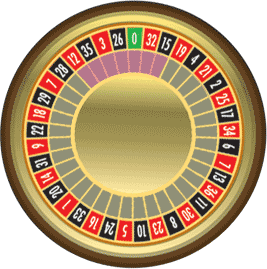
\includegraphics[scale=.38]{Roulette}
\begin{itemize}
\item Roulette wheel has slots numbered $1$--$36$
\columnbreak
\item American wheel also has slots $0$ and $00$
\item $18$~slots red, $18$~slots black, $0,00$ green
\item Can bet that ball stops on particular number
\item Bet called \alert{straight up}
\item If ball stops on that number, casino pays player
$35$ times bet
\item If not, casino keeps bet
\end{itemize}
\end{multicols}
\end{frame}

\begin{frame}{Straight up}
\begin{itemize}
\item Calculate expected proceeds from betting $\$1$
on a particular number, a \alert{straight up}
\item Wheel has $38$ spaces, each equally likely
\item So $\frac{1}{38}$ the probability of winning
\item $\frac{37}{38}$ the probability of losing
\item $35\left(\frac{1}{38}\right)
+\left(-1\right)\left(\frac{37}{38}\right)
\only<+->{=\frac{35-37}{38}}
\only<+->{=-\frac{2}{38}}
\only<+->{=-\frac{1}{19}}$
\item Thus $-\frac{1}{19}\approx -0.053$ the expected proceeds
\end{itemize}
\end{frame}

\begin{frame}{Street}
\begin{itemize}
\item Can also bet on three numbers
\item Bet called a \alert{street}
\item (Numbers must lie in same row of \alert{layout})
\item If ball stops on any of those numbers, casino
pays player $11$ times bet
\item Calculate expected proceeds from betting $\$1$ on a street
\item $11\left(\frac{3}{38}\right)+\left(-1\right)\left(\frac{35}{38}\right)
\only<+->{=-\frac{2}{38}}
\only<+->{\approx -0.053}$
\end{itemize}
\end{frame}

\begin{frame}{Rule for roulette payouts} 
\begin{itemize}
\item In general, players can bet on $n$
chosen numbers for any $n$
\item (Chosen numbers subject to arrangement of layout)
\item Casino pays $\frac{36}{n}-1$ times
bet if ball lands on one of chosen numbers
\item For example,
\[\begin{array}{l|c|l}
n&\frac{36}{n}-1&\text{Name}\\\hline
1&35&\text{straight up}\\
3&11&\text{street}\\
18&1&\text{red, black, even, odd}
\end{array}\]
\end{itemize}
\end{frame}

\begin{frame}
\begin{itemize}
\item If $0$ and $00$ were removed, would be $36$ rather than $38$ spaces
\item So $\frac{1}{36}$ the probability that ball stops on particular number
\item If bet contains $n$ numbers
\[\left(\frac{36}{n}-1\right)\frac{n}{36}
+\left(-1\right)\frac{36-n}{36}
\only<+->{=1-\frac{n}{36}-1+\frac{n}{36}}
\only<+->{=0}\]
\item Thus roulette would be fair, if not for extra spaces $0$ and $00$!
\item In long run, players would win nothing and casino would not profit
\end{itemize}
\end{frame}

\begin{frame}{Term life insurance (Exercise 55)}
\begin{itemize}
\item Insurance company offers \alert{ten year life
insurance policy}:
\begin{itemize}
\item Customer pays company $\$1500$ (the \alert{premium})
\item If customer dies during the ten years
(the \alert{term}) company pays customer's estate
$\$40,000$ but keeps premium
\item If customer survives ten years, company pays customer
nothing and keeps premium
\end{itemize}
\item Suppose $0.97$ the
probability that 30~year old male lives to age $40$ (or longer)
\item Morbid as it sounds, calculating such probabilities
the goal of \alert{actuarial science}
\item Calculate expected proceeds of company
\end{itemize}
\end{frame}

\begin{frame}
\begin{itemize}
\item $1500\left(.97\right)+\left(1500-40000\right)\left(.03\right)
\only<+->{=300}$
\item Instead of $\$1500$ calculate \alert{minimum}
premium $P$ such that company profits in long run
\item[]
\begin{align*}
P\left(.97\right)+\left(P-40000\right)\left(.03\right)&>0\\
.97P+.03P-40000\left(.03\right)&>0\\
P&>40000\left(.03\right)=1200
\end{align*}
\item So for any $P>1200$ company expects to profit
\item Indeed, $300$ the expectation when $P=1500$
\end{itemize}
\end{frame}

\begin{frame}{Lawsuit (Exercise 50)}
\begin{itemize}
\item Client considering bringing lawsuit against a chemical company
\item Her lawyer estimates $70\%$ chance she wins $\$60,000$
\item $10\%$ chance she wins nothing
\item $20\%$ chance she loses case, pays $\$30,000$ in legal fees
\item Calculate expected gain or loss if client proceeds with case
\item $60000\left(0.7\right)
+0\left(0.1\right)-30000\left(0.2\right)
\only<+->{36000}$
\end{itemize}
\begin{remark}
\begin{itemize}
\item Experiment has \alert{three} outcomes, unlike previous examples
\item Expectation gives net proceeds \alert{on long run}
\item However, in lawsuit example, experiment only run once,
so expectation not helpful here
\end{itemize}
\end{remark}
\end{frame}

\end{document}
